\section[AMBIENTE DE ESTUDO]{AMBIENTE DE ESTUDO}

Como este trata de um projeto de desenvolvimento de software na área de análise de marcha, dois ambientes de trabalho distintos foram amplamente utilizados. São estes:

\begin{enumerate}
	\item Laboratório de Informática em Saúde (LIS) na Faculdade Gama (FGA) da Universidade de Brasília (UnB);
	\item Laboratório de Performance Humana (LPH) na Faculdade Ceilândia (FCE) da UnB.
\end{enumerate}

No LIS foram desempenhadas as tarefas relativas a engenharia de software e disponibilização do software.
Foram utilizadas estações de trabalho do tipo \emph{Power Mac} com sistema operacional \emph{MAC OS X} 10.10.3, sendo que uma foi preparada para funcionar como servidor de aplicação e roteador de rede. 
A estação preparada, serve de hospedeira de duas máquinas virtuais (\emph{Virtual Machines} - VMs) rodando através do software \emph{Virtualbox} 4.3. 
Cada VM utiliza sistema operacional \emph{Debian Wheezy GNU/Linux}. 
Uma destas VMs foi configurada como roteador e \emph{firewall} e a outra como servidor de aplicações.  
Outra estação de trabalho \emph{Power Mac} idêntica e um notebook rodando \emph{Ubuntu 14.04 GNU/Linux} foram utilizados como máquinas de desenvolvimento.
Um diagrama da rede criada no LIS é mostrado na figura \ref{lis_rede}.

\begin{figure}[ht]
	\centering
	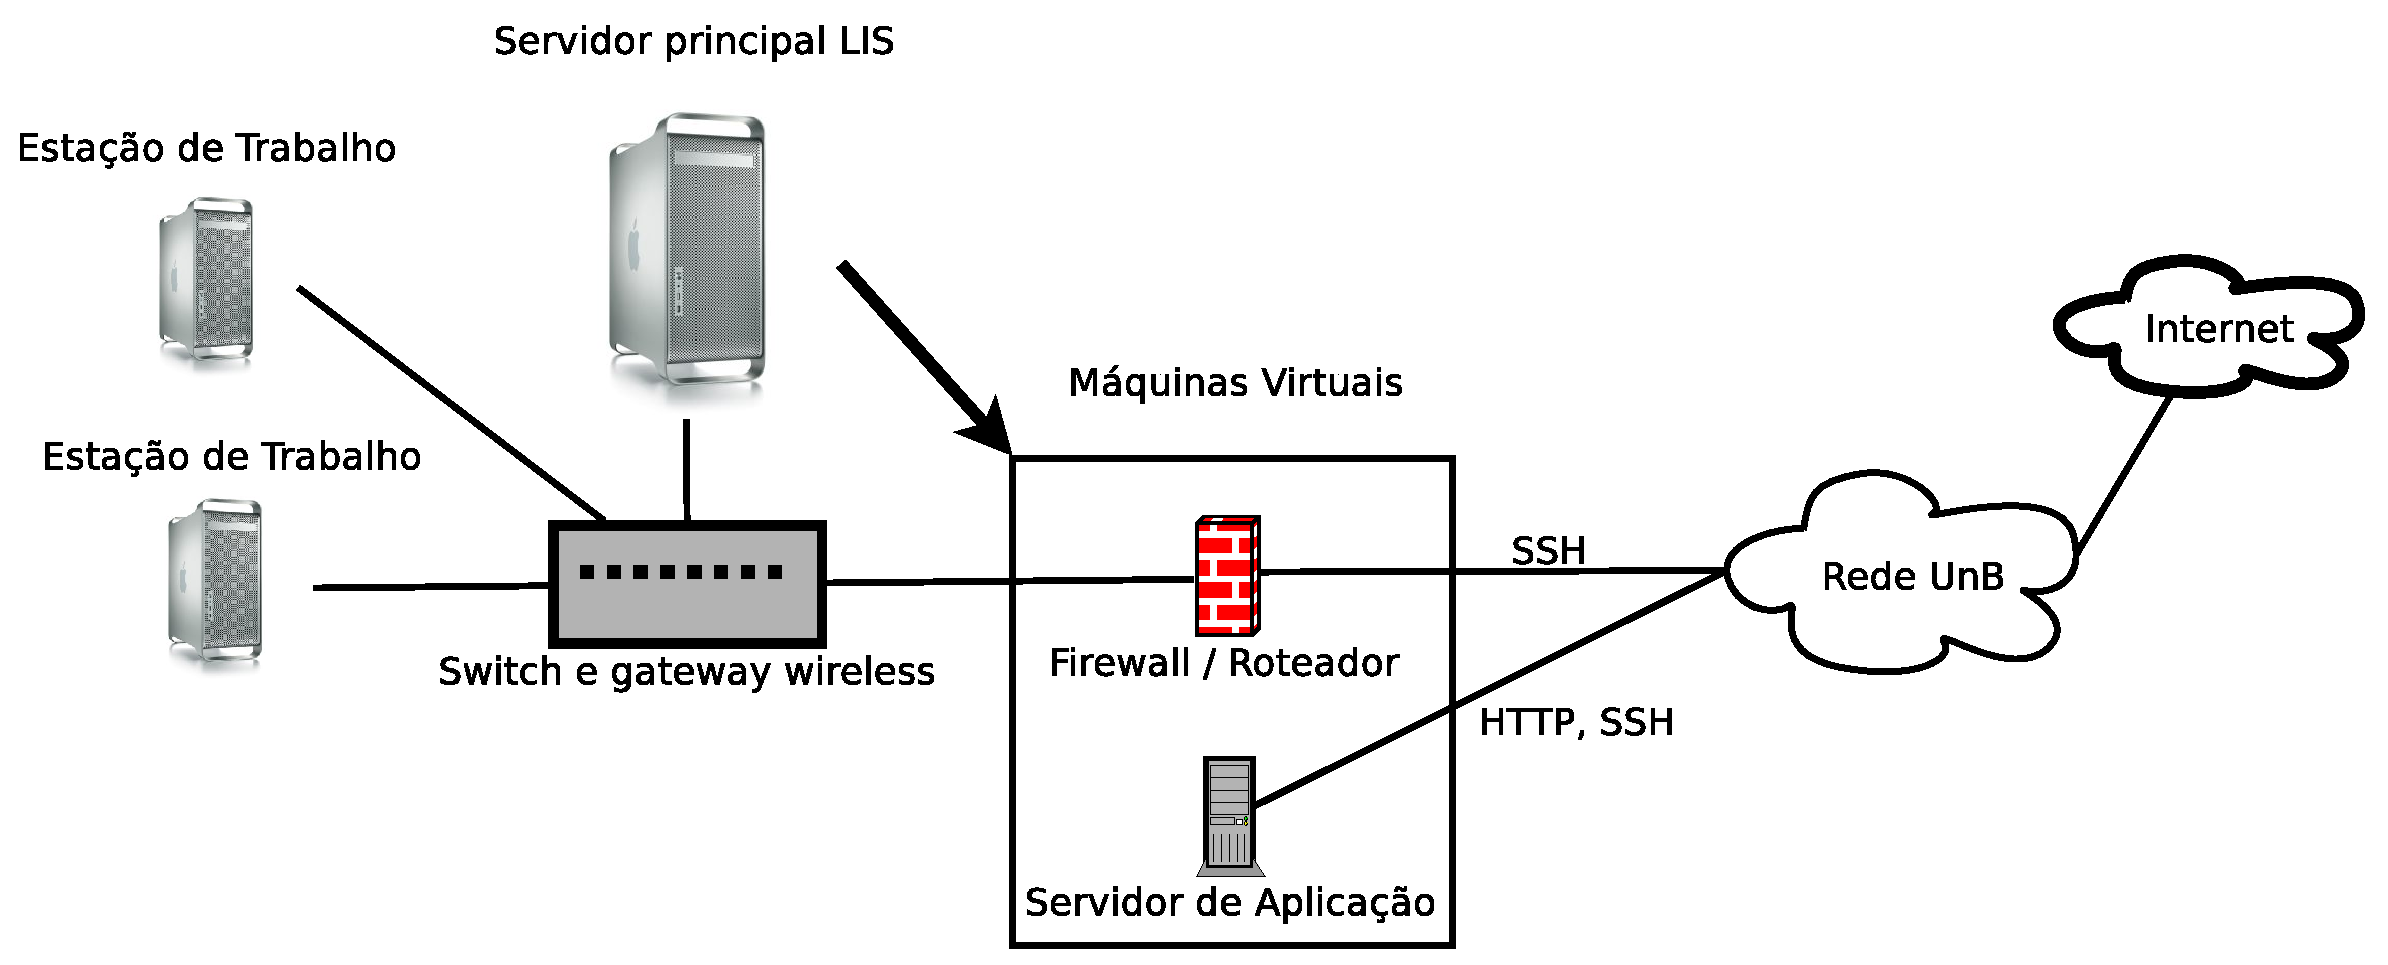
\includegraphics[width=15cm]{figuras/lis_rede.eps}
	\caption{Rede LIS}
	\label{lis_rede}
\end{figure}

O LPH foi utilizado para captura de dados de marcha humana. Este laboratório está equipado para coletar dados de plataformas de força, eletromiógrafos e de marcadores posicionados no corpo do paciente através de câmeras de vídeo (\emph{Motion Capture} - MOCAP). Para este trabalho foi utilizado o software \emph{QTM 3.2} da \emph{Qualisys}. 
